% !TEX root = main.tex

\chapter{Learning the functions of fission yeast proteins}
\label{chapter:yeast}

% \section*{Abbreviations}\label{abbreviations}
% \addcontentsline{toc}{section}{Abbreviations}

% \begin{table}[ht!]
%     \centering
%     \begin{tabular}{ll}
%         \toprule
%         \textbf{Abbreviation} & \textbf{Phrase} \\ \midrule
%         AUPR & area under the precision-recall curve \\
%         CAFA & Critical Assessment of Functional Annotation \\
%         E-value & expect value \\
%         FDR & false discovery rate \\
%         FWER & family-wise error rate \\
%         FYPO & Fission Yeast Phenotype Onotology \\
%         GO & Gene Ontology \\
%         HMM & hidden Markov model \\
%         RF & random forest \\
%         \emph{S. pombe} & \emph{Schizosaccharomyces pombe} \\
%         STRING & Search Tool for the Retrieval of Interacting Genes/Proteins \\
%         UPGMA & unweighted pair group method using arithmetic averages \\
%         \bottomrule
%     \end{tabular}
% \end{table}

\section{Introduction}

In this chapter, we develop a machine learning model to predict protein function using a combination of network, evolutionary and phenomics data. We train machine learning models using protein network embeddings from \ref{chapter:network-fusion}, evolutionary family data from CATH-FunFams and phenomic data from high-throughput phenomics screens of \emph{Schizosaccharomyces pombe} (\emph{S. pombe}; fission yeast) gene deletion mutants. First we analyse the phenomics data, then rigorously benchmark the machine learning models, before predicting functions of \emph{S. pombe} proteins. Finally, we enter our predictions into the Critical Assessment of Functional Annotation (CAFA) evaluation of protein function prediction methods. We begin the Introduction with pertinent information about fission yeast, phenomics screening and CAFA.

\subsection{\emph{Schizosaccharomyces pombe}}

\emph{S. pombe} is a unicellular eukaryotic species from the Fungi kingdom, and is \emph{probably the best model organism in the world} \cite{Bahler2006}. Fission yeast was first described in `pombe', the Swahili word for a type of beer produced in East Africa. The standard laboratory strain was isolated from wine grapes in French viticulture \cite{Jeffares2015}. The natural habitat of fission yeast is not known, but it is now found throughout the world in association with many human activities \cite{Jeffares2015}.

The `other' yeast \emph{Saccharomyces cerevisiae} (\emph{S. cerevisiae}; budding yeast) replicates asexually by budding---an asymmetric variant of mitosis \cite{Goffeau1996}. Whilst \emph{S. pombe} also replicates asexually, its cells divide symmetrically by binary fission in a process that is more similar to mammalian mitosis \cite{Hoffman2015}. \emph{S. pombe} is usually haploid, but, in stressful situations, two haploid cells of opposite mating types can fuse to form a diploid cell, which then divides into four haploid spores \cite{Egel1989}.

The \emph{S. pombe} genome is composed of $13.8$ Mb of DNA across three chromosomes \cite{Wood2002}. Phylogenetics reveals that fission yeast diverged from budding yeast \numrange{330}{420} million years ago, which makes the two yeasts as different to each other as animals are to either \cite{Sipiczki2000}. Fission yeast has $338$ genes that are conserved in humans, but absent in budding yeast, which is almost twice as many as the $179$ budding yeast genes that have orthologs in humans, but are absent in fission yeast \cite{Hoffman2015}. As such, fission yeast is an ideal model of eukaryotic cellular processes \cite{Nurse1976}.

Functional genomics in \emph{S. pombe} has been aided by the generation of a library of haploid gene deletion strains for all non-essential genes \cite{Kim2010}. Each gene was replaced with a selectable KanMX marker that allows for positive selection of the knockout strains. Short oligonucleotide sequences, known as barcodes, flank the marker with a unique sequence for each knocked out gene. All barcodes can be amplified by the polymerase chain reaction simultaneously using universal sequences. This allows strains to be profiled in a parallel and competitive fashion using Bar-seq \cite{Han2010,Smith2009}, or barcode sequencing.

\subsubsection{Function annotations}

Since 1992, when the budding yeast genome was sequenced, the percentage of functional characterisation of its proteome initially increased rapidly, but over the past decade has plateaued at $82\%$ \cite{Wood2019}. Fission yeast saw a much faster increase over a shorter time frame, but it too has topped out at $84\%$ coverage \cite{Wood2019}. Biological roles for the remaining $\sim 20\%$ of proteins remain elusive. Strangely, many of these proteins are conserved in humans, which suggests that they are involved in key cellular processes and therefore are a priority to study \cite{Wood2019}. There are many reasons why a protein may not have been studied \cite{Stoeger2018}, ranging from biological biases (experimental assays, detectability of functions, cost effectiveness) to cultural biases (funding priorities, citability, fashion trends). Next, we touch on some explanations for these biases.

Yeast gene deletion mutants that are unable to grow in standard laboratory conditions on rich media are deemed to be `essential' genes. In fission yeast, there are \num{1390} essential genes, found by searching PomBase \cite{Lock2018} for `inviable cell population' (Fission Yeast Phenotype Onotology (FYPO) \cite{Harris2013} term FYPO:0002059; null expression, single allele genotypes) on March 23, 2020. Of the non-essential genes in budding yeast, $34\%$ of gene deletion mutant strains show a growth phenotype when grown in standard conditions, but $97\%$ of genes are essential for normal growth in at least one of \num{1144} different chemical genomic assays \cite{Hillenmeyer2008}. The remaining $3\%$ of genes that did not display a phenotype may do so in at least one condition that has not (yet) been tested. Experimental function annotations are known to be biased towards high-throughput assays that are able to generate large volumes of functional annotations for many proteins (see \ref{sec:phenomics} for an example), but usually only for a tight range of functions \cite{Schnoes2013}. Furthermore, these annotations are usually subject to the curse of `few articles, many proteins', whereby $0.14\%$ of papers in the Gene Ontology Consortium account for the annotations of $25\%$ of proteins \cite{Schnoes2013}. Functional annotations derived from high-throughput experiments have a high error rate, so would benefit from being confirmed by independent high-throughput studies, or targeted low-throughput experimental validation. As such, the degree to which we can trust functional annotations, across all species, is questionable. We explore the scope of opportunities for protein function prediction in \emph{S. pombe} in \ref{sec:fission-yeast-known-functions} by analysing Gene Ontology terms annotated to proteins. Finally, the law of diminishing returns suggests that publishing papers on highly studied proteins such as p53 (that has amassed over \num{33000} publications since 2007 \cite{Wood2019}) will not be as fruitful as investigating a conserved human protein whose orthologues in any species have not been characterised.

\subsubsection{Function prediction}

A previous joint PhD project between the Orengo and Bähler groups involved the development of Compass, a method to predict \emph{S. pombe} protein function using protein networks. Using the \emph{S. pombe} Search Tool for the Retrieval of Interacting Genes/Proteins (STRING) network \cite{Szklarczyk2015}, weighted adjacency matrices were generated for each of the seven edge types: `neighborhood', `fusion', `cooccurence', `coexpression', `experimental', `database' and `textmining' (see \ref{network-data} for details). These adjacency matrices were summed to form a combined graph---a cheap and cheerful data fusion technique. To account for false negative and false positive edges, a kernel function was applied to the adjacency matrix to generate a kernel matrix. In this case, the commute-time kernel \cite{Fouss2012} was generated, which represents the expected number of steps it would take to travel from node $v_i$ to $v_j$ and return back to $v_i$ in a random walk on graph nodes. The commute-time is not only able to measure distances between nodes, but is also able to capture topological features of the graph's wiring pattern at mesoscopic resolution. This is beneficial because the Bähler group has previously shown that topological features of \emph{S. pombe} functional networks are predictive of protein function \cite{Sarac2012,Pancaldi2012}. Network commute-times, and kernels thereof, were used previously by the Orengo group to successfully predict protein function in a guilt-by-association framework using combinations of kernels to fuse heterogenous data and kernel matrices to measure the similarity between pairs of proteins \cite{Lees2015,Heriche2014}. Lehtinen \emph{et al.} \cite{Lehtinen2015} used kernel matrices to train a supervised partial least squares regression model \cite{Cristianini2004} to predict protein function by supervised learning. Partial least squares regression first learns a low-dimensional representation of the kernel matrix, in a similar manner to dimensionality reduction into principal components, followed by ordinary least squares regression in this low-dimensional space.

Compass was benchmarked against GeneMANIA \cite{Franz2018}, the de facto method for protein function prediction at that time.
GeneMANIA is a network-based protein function prediction method. First, GeneMANIA combines multiple functional association networks by calculating a weighted average of the adjacency matrices. A ridge regression model (L2 regularised linear regression) is trained to learn the weightings for each network, with the ability to downweight redundant and irrelevant information. Then, GeneMANIA runs label propagation on the composite network to predict protein function. The label propagation algorithm takes a set of seed proteins, a set of positive examples (positive node bias), and optionally a set of negative examples (negative node bias). Labels are propagated through the network in an optimisation process guided by a cost function that tries to minimise the difference between the label of neighbouring nodes and also the difference between the predicted label and the initial bias for each node. Compass consistently outperformed GeneMANIA on a variety of benchmarks and across a panel of metrics \cite{Lehtinen2015}.

The field of protein function prediction has seen rapid development and progress in the past decade, enabled by higher-quality data that covers more proteins and functions, and on the other hand by advances in machine learning methods and computational power, which together have produced more performant models. We make use of these advances in this study to make better predictions of \emph{S. pombe} protein function.

% \textbf{Ageing}
%
% Replicative lifespan is defined as the maximum number of cell divisions a cell can undergo. In budding yeast replicative lifespan is measured by removing daughter cells that are easily distinguished from mother cells and measuring how many times the the mother is able to divide \cite{Kaeberlein2010}. Usually cells manage approximately 20 divisions \cite{MORTIMER1959}. Replicative lifespan is harder to follow in fission yeast because division is morphologically symmetric. Jazwinski hypothesised in 1993 that for budding yeast `asymmetric reproduction of yeast cells lies at the foundation of yeast ageing and yeast longevity' \cite{Jazwinski1993}. The first sign that fission yeast also divide asymmetrically, on some level, came with the observation that mother cells become larger and rounder after four divisions \cite{Barker1999}. Damaged proteins were then shown to accumulate asymmetrically during division \cite{Erjavec2008}. Both findings make logical sense: if truly symmetric division occurred, yeast cultures would die once the accumulated damage reached a critical threshold. Instead, fission yeast cultures are immortalised at the population level by segregating damaged proteins into ageing cells, whilst retaining functional proteins in replicating cells.
%
% Chronological lifespan is defined as the length of time that a cell can survive in a quiescent, non-dividing state. Chronological lifespan can be measured in yeast cultures whose cells have stopped dividing because their carbon source has been depleted. These cells are periodically introduced into new rich media to determine their ability to resume growth. When starved for a number of days cells are able to continue growing when nutrients are reintroduced, but this ability diminishes with time and ultimately ceases. Calorie restriction has been shown to increase chronological lifespan in fission yeast, demonstrating that glucose regulation controls ageing \cite{Roux2009}. In addition, chronological lifespan is also associated with mitochondrial activity, reactive oxygen species production, resistance to stress, proteasome activity and autophagy \cite{Lin2014}. Ageing genes have been discovered in fission yeast that extend chronological lifespan when they are knocked out of haploid cells \cite{Rallis2014,Sideri2014}. In this study, these so called anti-longevity genes are used as seeds to predict novel ageing genes using fusions.

\subsection{Phenomics}
\label{sec:phenomics}

Phenomics is the description and prediction of phenotypes in relation to genotypes \cite{Houle2010a}. Use of the term took off in 1999, when Schilling and colleagues explained that genome sequencing, proteomics, systems biology and bioinformatics have enabled large, heterogenous data sets to be interrogated to understand genotype-phenotype relationships \cite{Shuler1999,Schilling1999}. That year, an early commentary about the nascent field of proteomics suggested that phenomics is ``an all embracing term (on a par with genomics) to describe functional genomics'' \cite{Dove1999}. Phenomics screens are typically genome-wide high-throughput experiments that produce high-dimensional phenotypic data.

Some phenotypes have direct one-to-one relationships with their causal genotypes. Examples include fully penetrant mutations in the amyloid-β precursor protein that cause familial Alzheimer's disease (\ref{sec:Alzheimer's disease}), or Gregor Mendel's genetic hybridisation experiments in peas \cite{Mendel1866}. However, the majority of phenotypes are complex (meaning `multivariate', where more than one gene determines a phenotype) where there is no clear relationship between genotype and phenotype. It cannot be stated more succinctly than in \cite{Houle2010}

\begin{quote}
    Although genotypes exist and are inherited in a discrete space convenient for many sorts of analyses, the causation of key phenomena such as natural selection and disease takes place in a continuous phenotype space whose relationship to the genotype space is only dimly grasped.
\end{quote}

Obvious exemplary complex phenotypes include height, susceptibility to cancer, and rate of ageing. Despite the lack of a clear relationship between genotype and phenotype, it is clear that there \emph{is} a relationship.

Another way to think about complex phenotypes is that they are emergent properties \cite{Novikoff1945}. Genotypes gives rise to phenotypic units that are integrated, from which a complex phenotype may arise \cite{Murren2012}. Novikoff states in \cite{Novikoff1945} that

\begin{quote}
    Knowledge of the laws of the lower level is necessary for a full understanding of the higher level; yet the unique properties of phenomena at the higher level can not be predicted, a priori, from the laws of the lower level.
\end{quote}

In other words, phenomics can elicit higher level phenotypes and can predict which lower levels (genes or variants) should be investigated further.

Phenomics has become a popular tool in the geneticist's toolbox. For example, it has been used to study the effects of obesity in human \cite{Hoyles2018}, increase crop yields \cite{Zhao2019,Watt2020}, and understand mammalian gene function in mouse \cite{Brown2018a}. Over the next decade, many more genotype-phenotype relationships will need to be untangled now that gene editing has been trivialised with CRISPR-Cas9 \cite{Mali2013a,Cong2013}. Phenomics will likely play a key role \cite{Gerlai2002}.

Phenomics has also been an important tool for studying genotype-phenotype relationships in \emph{S. pombe} \cite{Rallis2016}. Genome-wide screens in fission yeast are facilitated by the Bioneer library of gene deletion strains for all non-essential genes \cite{Kim2010} and the ease with which quantitative phenotypes can be collected. A number of phenotypic proxies are used in \emph{S. pombe}, including automated colony-sizing of colonies grown on solid media with computational processing of the large volume of data \cite{Bischof2016,Zackrisson2016,Kamrad2020,Sailem2020}, or the abundance of barcodes in multiplexed Bar-seq experiments \cite{Smith2009,Romila2019}.

A common strategy is to screen strains in the presence of some stressor that elicits the conditional essentiality of genes. One study identified $33$ new ageing genes by inhibiting the TORC1 signalling pathway in the gene deletion mutant stain library with rapamycin and caffeine \cite{Rallis2014a}. Whilst it was known that a high dosage of caffeine is toxic to fission yeast, but a low dosage can be tolerated \cite{Gentner1975,Osman1998}, the genetic reasons were unknown. A second screen of the gene deletion mutant stain library in media containing caffeine found that oxidative stress pathways are responsible for tolerance \cite{Calvo2009}. A third study identified $60$ new genes by screening the gene deletion mutant strain library in the presence of the transcriptional inhibitor 6‐azauracil \cite{Zhou2015a}.

\subsection{CAFA 4}

The latest iteration of the CAFA protein function prediction challenge \cite{Radivojac2013,Jiang2016,Zhou2019}, CAFA 4, took place between October 2019 and February 2020. CAFA's organisers provide a set of target protein sequences, where the aim is for participants to predict the functions of these sequences. In CAFA4, the targets were whole proteomes from $18$ model organism species, including human, mouse, fly, worm, baker's yeast, and, crucially, fission yeast. Participants could predict functions from any of three disjoint ontologies: Gene Ontology, Human Phenotype Ontology \cite{Kohler2019}, and Disorder Ontology \cite{Hatos2020}, which was included for the first time. Viewed in its wider context, CAFA 4 ultimately aimed to improve the quality and coverage of functional annotations for a large number of important proteins in the biological sciences. Each participating team could enter predictions from three separate models, which were assessed for coverage using $F_{\max}$ (\ref{eqn:Fmax}) and (semantic) precision using $S_{\min}$ (\ref{eqn:Smin}). Teams were ranked according to their best performing model on each metric, which allows teams to enter a `strict' model that is optimised for $S_{\min}$ and a `relaxed' model for $F_{\max}$.

An initial evaluation of CAFA 4 took place and was presented at the ISMB conference in July 2020. The performance of the top $10$ models under $F_{\max}$ and $S_{\min}$ were presented for each of the three Gene Ontology (GO) name spaces. The final evaluation is expected to take place in November 2020, with a publication expected in mid-2021.

\subsubsection{Contributions}

Fission yeast is an important model organism to understand the biological mechanisms of cellular processes.
In this chapter, develop machine learning models that predict the functions of \emph{S. pombe} proteins.
To do this, we collected a large, phenomic data set of \emph{S. pombe} gene deletion mutant strains grown in $131$ different conditions.
Using an extensive array of analyses, we consistently found that the growth phenotypes were not reliable, reproducible or predictive of protein function.
We trained machine learning models using this bespoke experimental data, alongside orthogonal data from protein networks and evolutionary information from CATH.
We evaluated the performance of models trained on these data modes separately, and in combination, finding that the best performing model used a combination of network and evolutionary data.
In particular, we focussed on functions that were predicted for proteins conserved in vertebrates, and those that currently have no experimentally characterised functions in \emph{S. pombe}.
Finally, we entered the predictions from this model into the fourth CAFA evaluation of protein function prediction methods.

\section{Methods}

\subsection{Growth phenotyping}
\label{sec:methods-gp}

\subsubsection{Collection}

All genes have been systematically deleted from \emph{S. pombe}. Strains of the $\sim \num{3700}$ non-essential gene deletion mutants (out of \num{5137} genes in total) are available commercially as a library, known as the Bioneer library \cite{Kim2010}.

To measure the effect of gene deletions on the growth phenotype of \emph{S. pombe}, the library was plated onto agar media supplemented with different molecules. The plates were incubated at various temperatures and for various times to allow the colonies to grow. The particular combination of media, added molecules, temperature and incubation time is referred to as the `condition'. Growth phenotypes were collected from $131$ unique conditions. At an appropriate time point---when colony growth is not saturated, so that slow-growing colonies can be distinguished from fast-growing colonies---the plates are scanned.

The library was grown in \num{1536} colony format, spread across three plates. Plates exhibit spatial biases, especially at the edges where competition for resources is lower. Wild type strains are plated every four strains to form a grid that is used to correct colony sizes and remove spatial biases.

\subsubsection{Processing}

Plate images were processed using pyphe \cite{Kamrad2020}. pyphe was inspired by scan-o-matic \cite{Zackrisson2016}, a pipeline for processing plate-based high-throughput growth phenotyping experiments.

The grid of wild type colonies is used to interpolate a `reference surface' across the plate, corresponding to the expected growth of a wild type colony at any point on the plate. Colony sizes are normalised by dividing the colony size by the reference surface value for the colony's position on the plate. Colonies of gene deletion mutants that are less fit than wild type will have a relative colony size $<1$, whilst those that are fitter will have a relative colony size $>1$.

In total, \num{2832384} colonies were present in the data set (\ref{fig:processing-steps}). Colonies were removed from the data set if:

\begin{itemize}
    \item gene ID is `grid' or `empty'
    \item colony size, reference surface, or colony circularity is missing
    \item colony size, corrected colony size, or reference surface $\le 0$
\end{itemize}

\num{2389858} colonies remained after `grid' and `empty' colonies were removed (\ref{fig:processing-steps}). \num{2256475} colonies remain after poor-quality colonies were removed. Sizes were rounded to $3$ decimal places to remove excess numerical precision that is probably experimental noise. Phloxine B is a red food dye that is used in yeast cell-viability assays \cite{Noda2009}. Cell membranes prevent the dye from entering cells, however, when cells die and membrane integrity is lost, the dye enters cells. Colonies that were grown in conditions with, and without, phloxine B were pooled because phloxine B does not interfere with growth. Colony sizes for each strain were normalised, to remove effects that knocking out the gene may have on growth, by dividing by the mean colony size of the strain in plain media at $32$$^{\circ}$C: `YES\_32' for conditions based on YES media, or `EMM\_32' for EMM media. Colony sizes were $\log_2$-transformed to make inverse growth differences symmetric about $0$. For example, $\log_2(2) = 1$ and $\log_2(2^{-1}) = \log_2(0.5) = -1$. Each strain-condition pair was then represented by the colony whose size that was most different to the wild type by

\begin{equation}
    \label{eqn:argmax_abs}
    X[\text{argmax}(\text{abs}(X))].
\end{equation}

Finally, for each condition, any missing colony sizes were imputed using the mean colony size of strains in that condition. Mean imputation was chosen so that imputed values would not have any effect when training machine learning models. From now on, we use the term `colony size' to refer to colony sizes that are normalised and $\log_2$-transformed for brevity.

\subsubsection{Significance testing}

Phenotype hits were called using null hypothesis significance testing. Absence of knocked out genes may affect growth---often negatively---regardless of the condition. To account for these effects, the null distribution for each strain is the distribution of its colony sizes in plain media at $32$$^{\circ}$C: `YES\_32' for conditions based on YES media, or `EMM\_32' for EMM media. For each strain and condition, the colony size distribution was compared to its corresponding null distribution using the two-sample unequal variance t-test (also known as Welch's test). The null hypothesis was that there is no difference between how a strain grows in a condition and its corresponding control condition.

$P$ values were corrected for multiple testing using the Benjamini-Hochberg method \cite{Benjamini1995}, which controls the false discovery rate (FDR), i.e. the expected proportion of rejected $H_0$s that are true. FDR methods provide less strict control of type I errors---rejection of a true $H_0$, a false positive---but have higher power---the probability that $H_0$ is rejected when $H_1$ is true. The Benjamini-Hochberg method first sorts the $P$ values $P_1, P_2, ..., P_J$. For a given significance threshold $\alpha$, the first $j$ hypotheses are rejected for which $P_j \le \frac{\alpha j}{J}$.

The Bonferroni method \cite{Dunn1961,Dunn1959} controls the family-wise error rate (FWER), i.e. the probability of making at least one type I error (false positive rate). The Bonferroni method rejects all hypotheses for which $P_j < \frac{\alpha}{J}$. For $J$ hypothesis tests, the FWER at a given significance threshold $\alpha$ is $1-(1-\alpha)^J$. For example, at the $0.01$ significance level, if $100$ tests are performed, the FWER $= 1-0.99^{100} = 0.634$. In other words, there is a $63\%$ chance of making one or more type I errors. FWER methods provide strict control of type I errors, but have correspondingly low power. If it is desirable for the false positive rate (the type I error rate) to be low---for example hits are to be analysed manually---Bonferroni could be used. Conversely, if high power is more important, Benjamini-Hochberg could be used.

\subsection{Machine learning}

\subsubsection{GO Slim annotations}

The Gene Ontology \cite{TheGeneOntologyConsortium2015} `2018-11-12' release was downloaded on November 14, 2018. \emph{S. pombe} GO annotation data `10/15/2018' release was downloaded from PomBase \cite{Lock2018} on November 14, 2018. The $53$ \emph{S. pombe} GO Slim terms were accessed from PomBase on November 14, 2018 (https://www.pombase.org/browse-curation/fission-yeast-go-slim-terms). GO Slim terms were chosen as targets, as these terms are chosen to be sufficiently informative terms in the ontology.

The GO annotation targets for machine learning were constructed as an $[n\text{ genes} \times m\text{ terms}]$ binary matrix. For each gene and GO Slim term pair, the corresponding position in the matrix is set to $1$ if the gene is annotated with the term, or any of its descendant (more specific) terms in the ontology, else $0$. The following relationships were considered: `is\_a', `part\_of', `regulates', `positively\_regulates' and `negatively\_regulates'. Only high-quality annotations with experimental (EXP, IDA, IPI, IMP, IGI or IEP) or curated (ISS, ISO, ISA, ISM, IGC, IBA, IBD, IKR, IRD, RCA, TAS or IC) evidence codes were considered. To avoid circularity, automatically assigned annotations with evidence code IEA were not considered.

For each of the three ontologies---biological process, molecular function and cellular component---the numbers of genes that have at least one annotation were counted. We consider there to be a hierarchy of preference for evidence codes of GO term annotations, starting with the `experimental' class (consisting of the evidence codes EXP, IDA, IPI, IMP, IGI, IEP, HTP, HDA, HMP, HGI and HEP), followed by `curated' (ISS, ISO, ISA, ISM, IGC, IBA, IBD, IKR, IRD, RCA, TAS and IC), `automatic' (IEA), and ending with undesirable annotations from the `bad' class (NAS and ND). We assign genes to evidence code classes using a fast and frugal tree \cite{Martignon2005,Raab2015}, that asks a total of $n$ questions and has $n+1$ exits---as opposed to classical decision trees that have $n^2$ exits \cite{Raab2015}. For each gene, $g$, we begin at the first internal node of the tree by asking the question ``does $g$ have at least one `experimental' annotation?'' If so, we assign it to the `experimental' class and exit the tree; if not, we proceed sequentially to the `curated', `automatic' and `bad' classes, exiting the tree if the question at each internal node evaluates to true.

\subsubsection{FunFam assignments}

All \num{5137} protein sequences encoded by the \emph{S. pombe} genome were downloaded from PomBase \cite{Lock2018} in FASTA format on February 21, 2019. Proteins were assigned to FunFams \cite{Das2015b} by searching their sequences against the FunFam hidden Markov model (HMM) library using hmmsearch from HMMER3 \cite{Mistry2013} and a threshold of E $< 10^{-3}$. In total, \num{3319} sequences had \num{149099} hits to \num{23900} FunFams.

Expect values (E-values) were $-\log_{10}$-transformed to convert to a linear scale. Multiplying by $-1$ means that good FunFam hits with low E-values have high feature values and weak hits with high E-values have low feature values---although the sign of features is not important for the random forest classifier used in this work. For machine learning, these data were converted to an $[n \text{ proteins} \times m \text{ FunFams}]$ matrix, with $99.8\%$ sparsity, $(1 - \frac{\num{149099}}{\num{3319}*\num{23900}}) * 100$.

Because \num{23901} FunFams were hit, the feature matrix is very wide---at least from a machine learning perspective. So, when predicting some GO term $g$, models were trained on FunFams that contain at least one protein annotated with $g$. GO \cite{TheGeneOntologyConsortium2015} annotations for all UniProt \cite{Bateman2019} accessions contained in FunFams were downloaded in February 2020. All annotations were included, except those with NAS, ND, TAS or IEA evidence codes, but UniProtKB-kw IEA curated terms were included. GO terms were associated with FunFams by identifying all GO terms that are annotated to proteins in each FunFam. Ancestor terms that have `is\_a', `has\_part', `part\_of' and `regulates' relationships were also included.

When predicting GO terms using only FunFam data, the \num{23900} FunFams that had at least one \emph{S. pombe} homologue were used as features.

\subsubsection{Network embeddings}

% (\ref{fig:pombe-loss})
Network embeddings of \emph{S. pombe} genes in networks from the STRING \cite{Szklarczyk2017} database were produced by a multimodal deep autoencoder (see \ref{chapter:network-fusion} and \ref{sec:results-pombe} for details). The $256$D embeddings were used from the $256$-$256$ architecture that produced the lowest validation loss.
Machine learning models were trained using the values in each dimension of the embedding as features.

\subsubsection{Random forests}

Supervised machine learning was used to predict GO annotations for \emph{S. pombe} proteins using random forests (RF) \cite{Murphy2012}. For an introduction to RFs, see (\ref{sec:intro-rf}). The RF implementation used in DecisionTree.jl builds forests of classification and regression trees (CART). We initially experimented with $100$ trees and later increased this to $500$ trees for final model evaluation. There is usually only a mild improvement in the performance when increasing from $100$ to $500$ trees ($<0.1$ AUPR improvement). The cost function used in this study employed the following criteria:

\begin{itemize}
    \item No maximum depth, so trees could grow arbitrarily deep.
    \item A minimum of two samples is needed to split a node, resulting in terminal nodes with single samples in each.
    \item No minimum purity increase, here defined according to minimising entropy.
\end{itemize}

Trees were not pruned in this study.

To better compare the performance using different input data, we implemented a strategy to obtain the same train-tests splits for each label and repeat, regardless of the input data. Before predicting the $i$th label in the $n$th repeat, the pseudo-random number generator is seeded with $i+n$ before being used to generate the cross-validation splits. However, if the input data does not contain the same set of strains (rows) as other input data, then the splitting strategy will not be the same.

Hyperparameters were chosen using an exhaustive grid search over the parameter ranges. Each combination of parameters was assessed using a nested five-fold stratified cross-validation. The parameter combination that produced the highest area under the precision-recall curve (AUPR) was chosen is shown in \ref{tab:hyperparameter-grid}.

\begin{table}[hbt!]
    \centering
    \caption{%
        RF hyperparameter optimisation.
        Hyperparameters that were optimised and the parameter ranges over which an exhaustive grid search was carried out are listed.
    }
    \label{tab:hyperparameter-grid}
    \begin{tabular}{llc}
        \toprule
        \textbf{Hyperparameter} & \textbf{Description} & \textbf{Parameter range} \\
        \midrule
        n\_subfeatures & Number of features used to grow each tree & $\{10, 25, 50, \sqrt{n} \} $ \\
        partial\_sampling & Proportion of examples used to grow each tree & $\{0.50, 0.75, 1.00\} $ \\
        \bottomrule
    \end{tabular}
\end{table}

Model performance was estimated using five-fold stratified cross-validation. The data was shuffled before each cross-validation. Five independent runs of cross-validation were performed to estimate the model performance under different train-test splits. Terms were predicted using the one-vs-rest multiclass strategy.

\subsubsection{Prediction}
\label{sec:rf-prediction}

After benchmarking, GO term annotations were predicted for \emph{S. pombe} genes. We took two approaches to do this. Initially, we used the canonical approach of training a model using all available training data, then predicting labels. Latterly, after realising that the random forest models had overfit on the training data and were conservative at predicting positive labels, we implemented a more liberal prediction strategy based on $5$-fold cross-validation. Under this strategy, models were trained using $80\%$ of the data and used to predict labels for the remaining $20\%$, and so on for each of the five train-test splits. This means that models are never trained on the same examples that they predict labels for, which forces models to predict labels using general principles that were learned in the training phase.

GO annotations were propagated to their parent terms in the GO DAG. Terms annotated to between $50$ and \num{1000} proteins were included in the target set, so that sufficient training examples were present for machine learning. Random forest classifiers were trained using $500$ trees. Because we did not use growth phenotype features to make final predictions, we did not exclude any genes from our data set. We observed that models were robust to values of hyperparameters, so for the sake of expediency, we did not perform hyperparameter optimisation. We chose sensible default values for the number of sub-features as $\sqrt{n}$ and partial sampling of $0.7$. GO terms were predicted using $5$-fold cross-validation. Predictive performance was evaluated using AUPR.


\subsubsection{CAFA}

CAFA is a protein function prediction challenge. Though similar to how GO terms were predicted for fission yeast, as explained in \ref{sec:rf-prediction}, a number of updates and modifications were made. STRING v11.0 \cite{Szklarczyk2019} was used. Due to potential circularity, the text mining STRING network was not included in prior benchmarks, but we included it here to boost our performance. $256$D network embeddings were generated using networks of the seven STRING edge types. The latest version of FunFams, v4.3, generated in January 2020, so were used. \emph{S. pombe} protein sequences were searched against the v4.2 and v4.3 FunFams using hmmsearch. GO terms associated with FunFams were downloaded in February 2020, and all terms, except those with NAS, ND, TAS and IEA, were included, as well as UniProtKB-kw IEA terms. CAFA provided a frozen version of the Gene Ontology for every team to use (October 7, 2019 release). Up-to-date \emph{S. pombe} GO annotations were downloaded from PomBase on January 14, 2020.

We experimented with many different combinations of features and submitted the three models that had the best AUPR from cross-validation. All three of the models were trained on the network embeddings. Additionally, v4.3 FunFams were used in model 1 and v4.2 FunFams in model 2. Inclusion thresholds were used for v4.2 FunFam HMMs, whereas, a threshold of E $< 10^{-4}$ was used for v4.3 FunFam HMMs to mitigate any potential over-splitting that may have occurred whilst generating these FunFams. E-values were $-\log_{10}$-transformed to be used as FunFam features.

Random forest predictions were post-processed. Parents of predicted terms were added with the same probability as the predicted term. GO taxon constraints were applied to remove terms that never occur in \emph{S. pombe}. Predictions were filtered to remove any duplicates and the prediction with the highest probability was kept. Predictions were submitted to CAFA 4 under the team name `OrengoFunFamLab2'.


\subsection{Data analysis}

\subsubsection{Clustering}

Growth phenotype data was clustered \cite{DHaeseleer2005} and heatmaps with dendrograms were plotted. Euclidean distance matrices were calculated \cite{Gibbons2002} (`euclidean' metric in \texttt{scipy.spatial.distance.pdist} \cite{Virtanen2020a}). The distance matrix was clustered using the unweighted pair group method using arithmetic averages (UPGMA) algorithm \cite{Sokal1958} (`average' method in \texttt{scipy.cluster.hierarchy.linkage} \cite{Virtanen2020a}). UPGMA performs bottom-up hierarchical agglomerative clustering to form a dendrogram by iteratively merging the two most-similar clusters. Distances between clusters are calculated as the mean distance between all pairwise combinations of items between each cluster. By considering all items in clusters, UPGMA is more robust to outliers than single-linkage clustering, which only considers the nearest pair of items. Heatmaps were plotted using \texttt{seaborn.clustermap}.

\subsubsection{Code}

Julia 1.1-1.4 was used for most of this work. Julia packages used were: DataFrames v0.19.1, DataFramesMeta v0.5.0, DecisionTree v0.10.1, Distances v0.8.0, GLM v1.1.1, HypothesisTests v0.8.0, MLBase v0.8.0, MLDataUtils v0.5.0, MultipleTesting v0.4.1, OBOParse v0.0.1, PlotlyJS v0.13.1, Plots v0.27.1, StatsBase v0.31.0, StatsPlots v0.10.2, and UMAP v0.1.4. Custom code is available as a Julia package PombeAgeingGenes.jl on GitHub (https://github.com/harryscholes/PombeAgeingGenes.jl). Python 3.7 was used to plot clustermaps of matrices using numpy v1.15.4, pandas v0.23.4, matplotlib v3.0.2 and seaborn v0.9.0.


\section{Results}

\subsection{Known functions of fission yeast proteins}
\label{sec:fission-yeast-known-functions}

Overarchingly, this project aims to accurately predict functions of \emph{S. pombe} genes, so that experimentalists can be informed about which targeted functional validations to perform, so as to increase the total number of genes with at least one `experimental' annotation, and to increase the total number of `experimental' annotations. \num{4523} ($88\%$) of \emph{S. pombe}'s \num{5137} protein-coding genes have at least one `experimental' annotation in any of the three ontologies---biological process, molecular function and cellular component (\ref{fig:evidence_codes_of_pombe_annotations}). However, if only biological process and molecular function terms are not considered, only \num{1963} ($38\%$) genes have at least one `experimental' annotation. This is because it is relatively easy to determine the subcellular location of proteins in high-throughput screens, such as automated fluorescence microscopy.

For the biological process and molecular function ontologies separately, \num{4190} ($82\%$) and \num{3310} ($64\%$) of genes have at least one high-quality annotation in the `experimental' or `curated' classes of GO evidence codes. In the cellular component ontology, \num{4449} ($87\%$) of genes have at least one `experimental' annotation, of which \num{2790} ($63\%$) are from high-throughput studies with evidence codes HTP, HDA, HMP, HGI or HEP, which may represent a significant bias in the functional distribution of \emph{S. pombe} gene annotations \cite{Schnoes2013}. Annotations in the `bad' class should not be trusted. Together with genes that have no annotations, there is an opportunity to assign functions from the biological process, molecular function and cellular component ontologies to $845$ ($16\%$), \num{1439} ($28\%$) and $231$ ($5\%$) genes, respectively.

\begin{figure}[!hbt]
    \centering
    \includegraphics[width=\textwidth]{./Chapter_yeast/evidence_codes_of_pombe_annotations}
    \caption{%
        Assessing the quality of GO term annotations in \emph{S. pombe} genes.
        For each ontology---biological process, molecular function and cellular component---together (All) and separately, \emph{S. pombe} genes are assigned to one of five classes---experimental, curated, automatic, bad and none---in that order of preference.
    }
    \label{fig:evidence_codes_of_pombe_annotations}
\end{figure}


\subsection{Colony size phenomics of fission yeast gene deletion mutants grown in a panel of conditions}

The growth phenotype data was processed as described in \ref{sec:methods-gp}. The entire data set contained \num{2832384} colonies. \num{2389858} colonies remained after `grid' and `empty' colonies were removed (\ref{fig:processing-steps}). \num{2256475} colonies remained after poor-quality colonies were removed. Some conditions were supplemented with a red food dye called phloxine B that is used in yeast cell-viability assays \cite{Noda2009}. The polar dye is excluded from healthy cells with intact membranes, but when membrane integrity is lost in dead cells, the dye is able to accumulate in cells and can be detected easily as red-stained colonies. In this way, dead cells can be distinguished from cells that are alive, but are unable to divide \cite{Mirisola2014}. Colonies that were grown in conditions that were, or were not, supplemented with phloxine B were pooled because phloxine B does not interfere with growth \cite{Kwolek-Mirek2014}.

\begin{figure}[!hbt]
    \centering
    \includegraphics{./Chapter_yeast/processing_steps}
    \caption{%
        Processing colonies in growth phenotype data.
        `All data': all colony size measurements in the data set,
        `All colonies': colonies remaining after `grid' and `empty' colonies were removed,
        `High-quality colonies': colonies remaining after poor-quality colonies were removed.
    }
    \label{fig:processing-steps}
\end{figure}

\subsection{Estimating the reliability of colony sizes}
\label{sec:Estimating the reliability of colony sizes}

For each strain-condition pair, the variance in colony size was calculated (\ref{fig:colony_sizes_variance}). Variances are distributed exponentially, with a heavy positive skew. Generally, strain-condition pairs have low variance, with mean $0.0733$ and \nth{95} percentile $0.287$.

\begin{figure}[!hbt]
    \centering
    \includegraphics{./Chapter_yeast/colony_sizes_variance}
    \caption{%
        Distribution of colony size variance across for all strain-condition pairs.
        Variance in colony size for strain-condition pairs with $> 1$ repeat were calculated.
    }
    \label{fig:colony_sizes_variance}
\end{figure}

We assessed the reliability of strain colony sizes from multiple repeats in the same condition. By reliability, we mean how similar are the sizes of pairs of colonies from the same strain grown in the same condition. We chose the condition `YES\_SDS\_0.04percent' because it had the most pairs of repeats, except for `YES\_32' and `EMM\_32'. Colony sizes from the \num{1055687} pairs of repeats for particular strains agreed poorly (\ref{fig:colony_sizes_reliability_YES_SDS_0.04percent}). These pairs of colony sizes had a Pearson correlation coefficient of $r = 0.215$. We also fitted a linear regression model to the pairs of colony sizes and found that this line deviates significantly from the ideal $y=x$ line---corresponding to perfect reliability---with a coefficient of determination $R^2 =0.036$.

\begin{figure}[!hbt]
    \centering
    \includegraphics{{{./Chapter_yeast/colony_sizes_reliability_YES_SDS_0.04percent}}}
    \caption{%
        Reliability of colony sizes.
        The condition `YES\_SDS\_0.04percent' was used.
        \num{1055687} pairs of repeats for particular strains exists.
        \num{20000} pairs were randomly sampled and plotted.
    }
    \label{fig:colony_sizes_reliability_YES_SDS_0.04percent}
\end{figure}

We observed that colonies of \emph{S. pombe} gene deletion mutants displayed a high false negative rate, i.e. a growth phenotype was not observed, despite the knocked out gene being affected by the growth condition.
In other words, strains would sometimes show a phenotype in one repeat, but inexplicably would not show any phenotype in other repeats.

Each strain-condition pair was then represented by the colony whose size had the largest effect size by \eqref{eqn:argmax_abs}. From now on, we refer to these values as the `colony size' for each strain-condition pair. Colony sizes across all strains and conditions follow a normal distribution with $\mathcal{N}(\mu = -0.046, \sigma^2=0.281)$ (\ref{fig:colony-sizes}). Mean colony size of $-0.046$ shows that strains tend not to have strong phenotypes in conditions, with a small trend towards being less fit. The variance of the fitted normal distribution agrees well with the empirical mean of colony size variance of each strain-condition pair (\ref{fig:colony_sizes_variance}).
Assuming normality, a standard deviation of $0.530$ means that $95\%$ of colonies will be within
\[
    \mu \pm 2\sigma = -0.046\pm 0.530 = -0.576 < x < 0.484.
\]
So taking the inverse logarithm results in $95\%$ of corrected colony sizes between
\[
    2^{-0.576}<x<2^{0.484} = 0.671<x<1.399.
\]

On closer inspection, the distribution is bimodal about $0$, due to the way that we calculated point estimates of colony sizes using $X[\text{argmax}(\text{abs}(X))]$. As the most extreme colony size, $x$, tends to zero, the probability, $P(x)$, also tends to zero,
\[
    \lim_{x \to 0} P(x) \to 0
\]
unless there is absolutely no phenotype, or no biological or technical error.

\begin{figure}[!hbt]
    \centering
    \includegraphics[width=0.9\textwidth]{./Chapter_yeast/colony_sizes_histogram}
    \caption{%
        Distribution of colony sizes from all strains and conditions.
        Colony sizes for all colonies (left) and $-0.5 \le x \le 0.5$ (right) are shown.
        Colony sizes were corrected using the reference surface from the grid of wild type colonies on each plate, normalised to the strain's growth in control conditions, and $\log_2$-transformed.
        Point estimates of the colony size distribution for each strain-condition pair, $X$, was calculated by $X \lbrack \text{argmax}(\text{abs}(X)) \rbrack$.
    }
    \label{fig:colony-sizes}
\end{figure}


\subsection{Identifying conditions that elicit strong phenotypes}

Conditions that elicit strong phenotypes were identified by calculating the mean colony size and variance per condition (\ref{fig:colony_sizes_mean_var}). In this context, strong phenotypes were defined as having mean colony size $> 0.2$ or $< -0.2$, or variance $> 1.0$. All of the three $10$ mM EGTA conditions had high variance $> 1.0$, along with EMM C (ciclopirox olamine, an antifungal drug) $2$ ug/ml. EGTA is a strong chelating agent that binds positively charged metallic magnesium and calcium ions. Conditions with small mean colony sizes were YES\_KCl\_0.5M\_SDS\_0.04percent and YES\_Diamide\_2mM.
$0.6$ M KCl decreases permeability of the \emph{S. pombe} cell membrane and increases its resistance to certain drugs \cite{Alao2015}, but \numrange{0.5}{2.0} M KCl interrupts logarithmic growth in \emph{S. cerevisiae} and is mutagenic \cite{Parker1990}. YES\_KCl\_0.5M\_SDS\_0.04percent had a mean colony size of $-0.270$, whereas, YES\_KCl\_1M\_SDS\_0.04percent on average were not affected as strongly and had mean colony size of $-0.035$. All other conditions with $0.04\%$ SDS did not have as strong effect sizes. Either, this is an outlier, or $0.05$ M KCl does not protect the cell membrane against detergent or acts synergistically to solubilise the membrane. Diamide is an oxidising agent that is toxic to \emph{S. pombe} at $3$ mM, and in the YES\_Diamide\_2mM condition, the mean colony size was $-0.208$.

\begin{figure}[!hbt]
    \centering
    \includegraphics{./Chapter_yeast/colony_sizes_mean_var}
    \caption{%
        Mean colony size per condition across all strains, against the variance.
        Conditions that elicit strong phenotypes, with mean colony size $>0.2$ or $< -0.2$, or variance $>1.0$, were labelled.
    }
    \label{fig:colony_sizes_mean_var}
\end{figure}

\section{Clustering strains and conditions according to phenotypic patterns}

% \todo{Function enrichment in clusters of proteins}

To identify groups of strains and conditions that had similar patterns of colony growth across all strains or all conditions, we clustered a $[\text{strains} \times \text{conditions}]$ matrix of colony sizes using Ward's method.
% For Ward figure:
The clustered heatmap is divided into two main clusters, where there smaller cluster at the bottom of the heatmap are sensitive to many conditions (\ref{fig:clustermap-ids-conditions}).
The larger cluster at the top of the heatmap are not affected by many conditions, or are resistant to certain blocks of conditions.
Many of the colonies in the lower cluster are also resistant to these conditions though, which is an interesting finding, as it shows that the wild type grows worse in these conditions than the gene deletion mutants.
The choice of media appears to affect the growth of colonies across the different strains, as shown by EMM-based conditions clustering into a block of conditions (pink), sandwhiched between YES-based conditions (green).

% For UPGMA figure:
% The clustered heatmap does not have much structure (\ref{fig:clustermap-ids-conditions}).
% The column and row dendrograms are step-like, with short branch lengths. This means that many conditions produce similar patterns of growth across all colonies and many strains have similar patterns of growth across all conditions. Consequently, leaves cannot be segregated easily into clades (subtrees).

% \todo{JB Doing the trigitization and omitting conditions where most mutants have no phenotypes should provide much better structured clusters. I thought you had done this at some point?}

\begin{figure}[!hbtp]
    \centering
    \includegraphics[width=0.95\textwidth]{./Chapter_yeast/clustermap_ids_conditions_trigitised}
    \caption{%
        Sensitivity of strains in conditions.
        A threshold of $1.25$-fold growth difference was set for resistant strains, where $\log_2(1.25) = 0.32$.
        Resistant colonies (yellow) have $\log_2$-transformed sizes $> 0.32$, and sensitive colonies (blue) have $\log_2$-transformed sizes $< -0.32$.
        The Euclidean distance matrix was clustered using Ward's method.
        Columns are coloured by media type, where green denotes YES media and pink denotes EMM media.
        % Colony sizes for all strains and conditions.
        % The Euclidean distance matrix was clustered using UPGMA.
        % Colony sizes were clamped to $\lbrack -2, 2 \rbrack$.
    }
    \label{fig:clustermap-ids-conditions}
\end{figure}

We also calculated correlation matrices for conditions (\ref{fig:clustermap-conditions}) and strains (\ref{fig:clustermap-ids}) and clustered these using UPGMA. The correlation matrix for conditions (\ref{fig:clustermap-conditions}) is the easiest of the three clustered heatmap figures to interpret because it is the smallest. Conditions based on EMM media cluster into two clades, that are not contaminated with any YES-based conditions. Furthermore, $11$ out of the $17$ EMM conditions can be easily separated from the remaining conditions in the first UMAP embedding dimension \cite{McInnes2018} (data not shown). UMAP is a dimensionality reduction method similar to, but more powerful than, principal component analysis. Most YES glucose conditions form a clade at the bottom right corner of (\ref{fig:clustermap-conditions}), with some contamination from other sugars (galactose, xilose and mannitol) and alcohols (glycerol and ethanol), which are metabolised similarly. Interestingly, although tea tree oil is a potent antifungal \cite{DAuria2001}, the two tea tree conditions also clustered into this clade. This is likely because all of these conditions result in small colonies.

\begin{figure}[!hbtp]
    \centering
    \includegraphics[width=\textwidth]{./Chapter_yeast/clustermap_conditions}
    \caption{%
        Correlation of conditions.
        The Pearson correlation coefficient (PCC) matrix of conditions across all strains was clustered using UPGMA.
    }
    \label{fig:clustermap-conditions}
\end{figure}

The study that identified tea tree as lethal to \emph{S. pombe} found the minimum inhibitory concentration to be $0.5\%$ v/v, but the conditions that we used were $0.25$ μl/ml and $0.50$ μl/ml, i.e. $5\%$ and $10\%$ of the minimum inhibitory concentration. Low concentrations of antibiotics are known to act as environmental signals for bacteria that cause multifarious cellular changes \cite{Bernier2013}. Although the mechanism of tea tree's antifungal properties is not known, it is thought to affect the permeability of membranes \cite{Mazu2016}. However, a tight clade was formed with the two tea tree conditions, YES\_glucose\_0.5percent\_32C and YES\_glucose\_1percent\_32C, so it is also possible that tea tree had a minimal effect on cells at such low concentrations.

\begin{figure}[!hbtp]
    \centering
    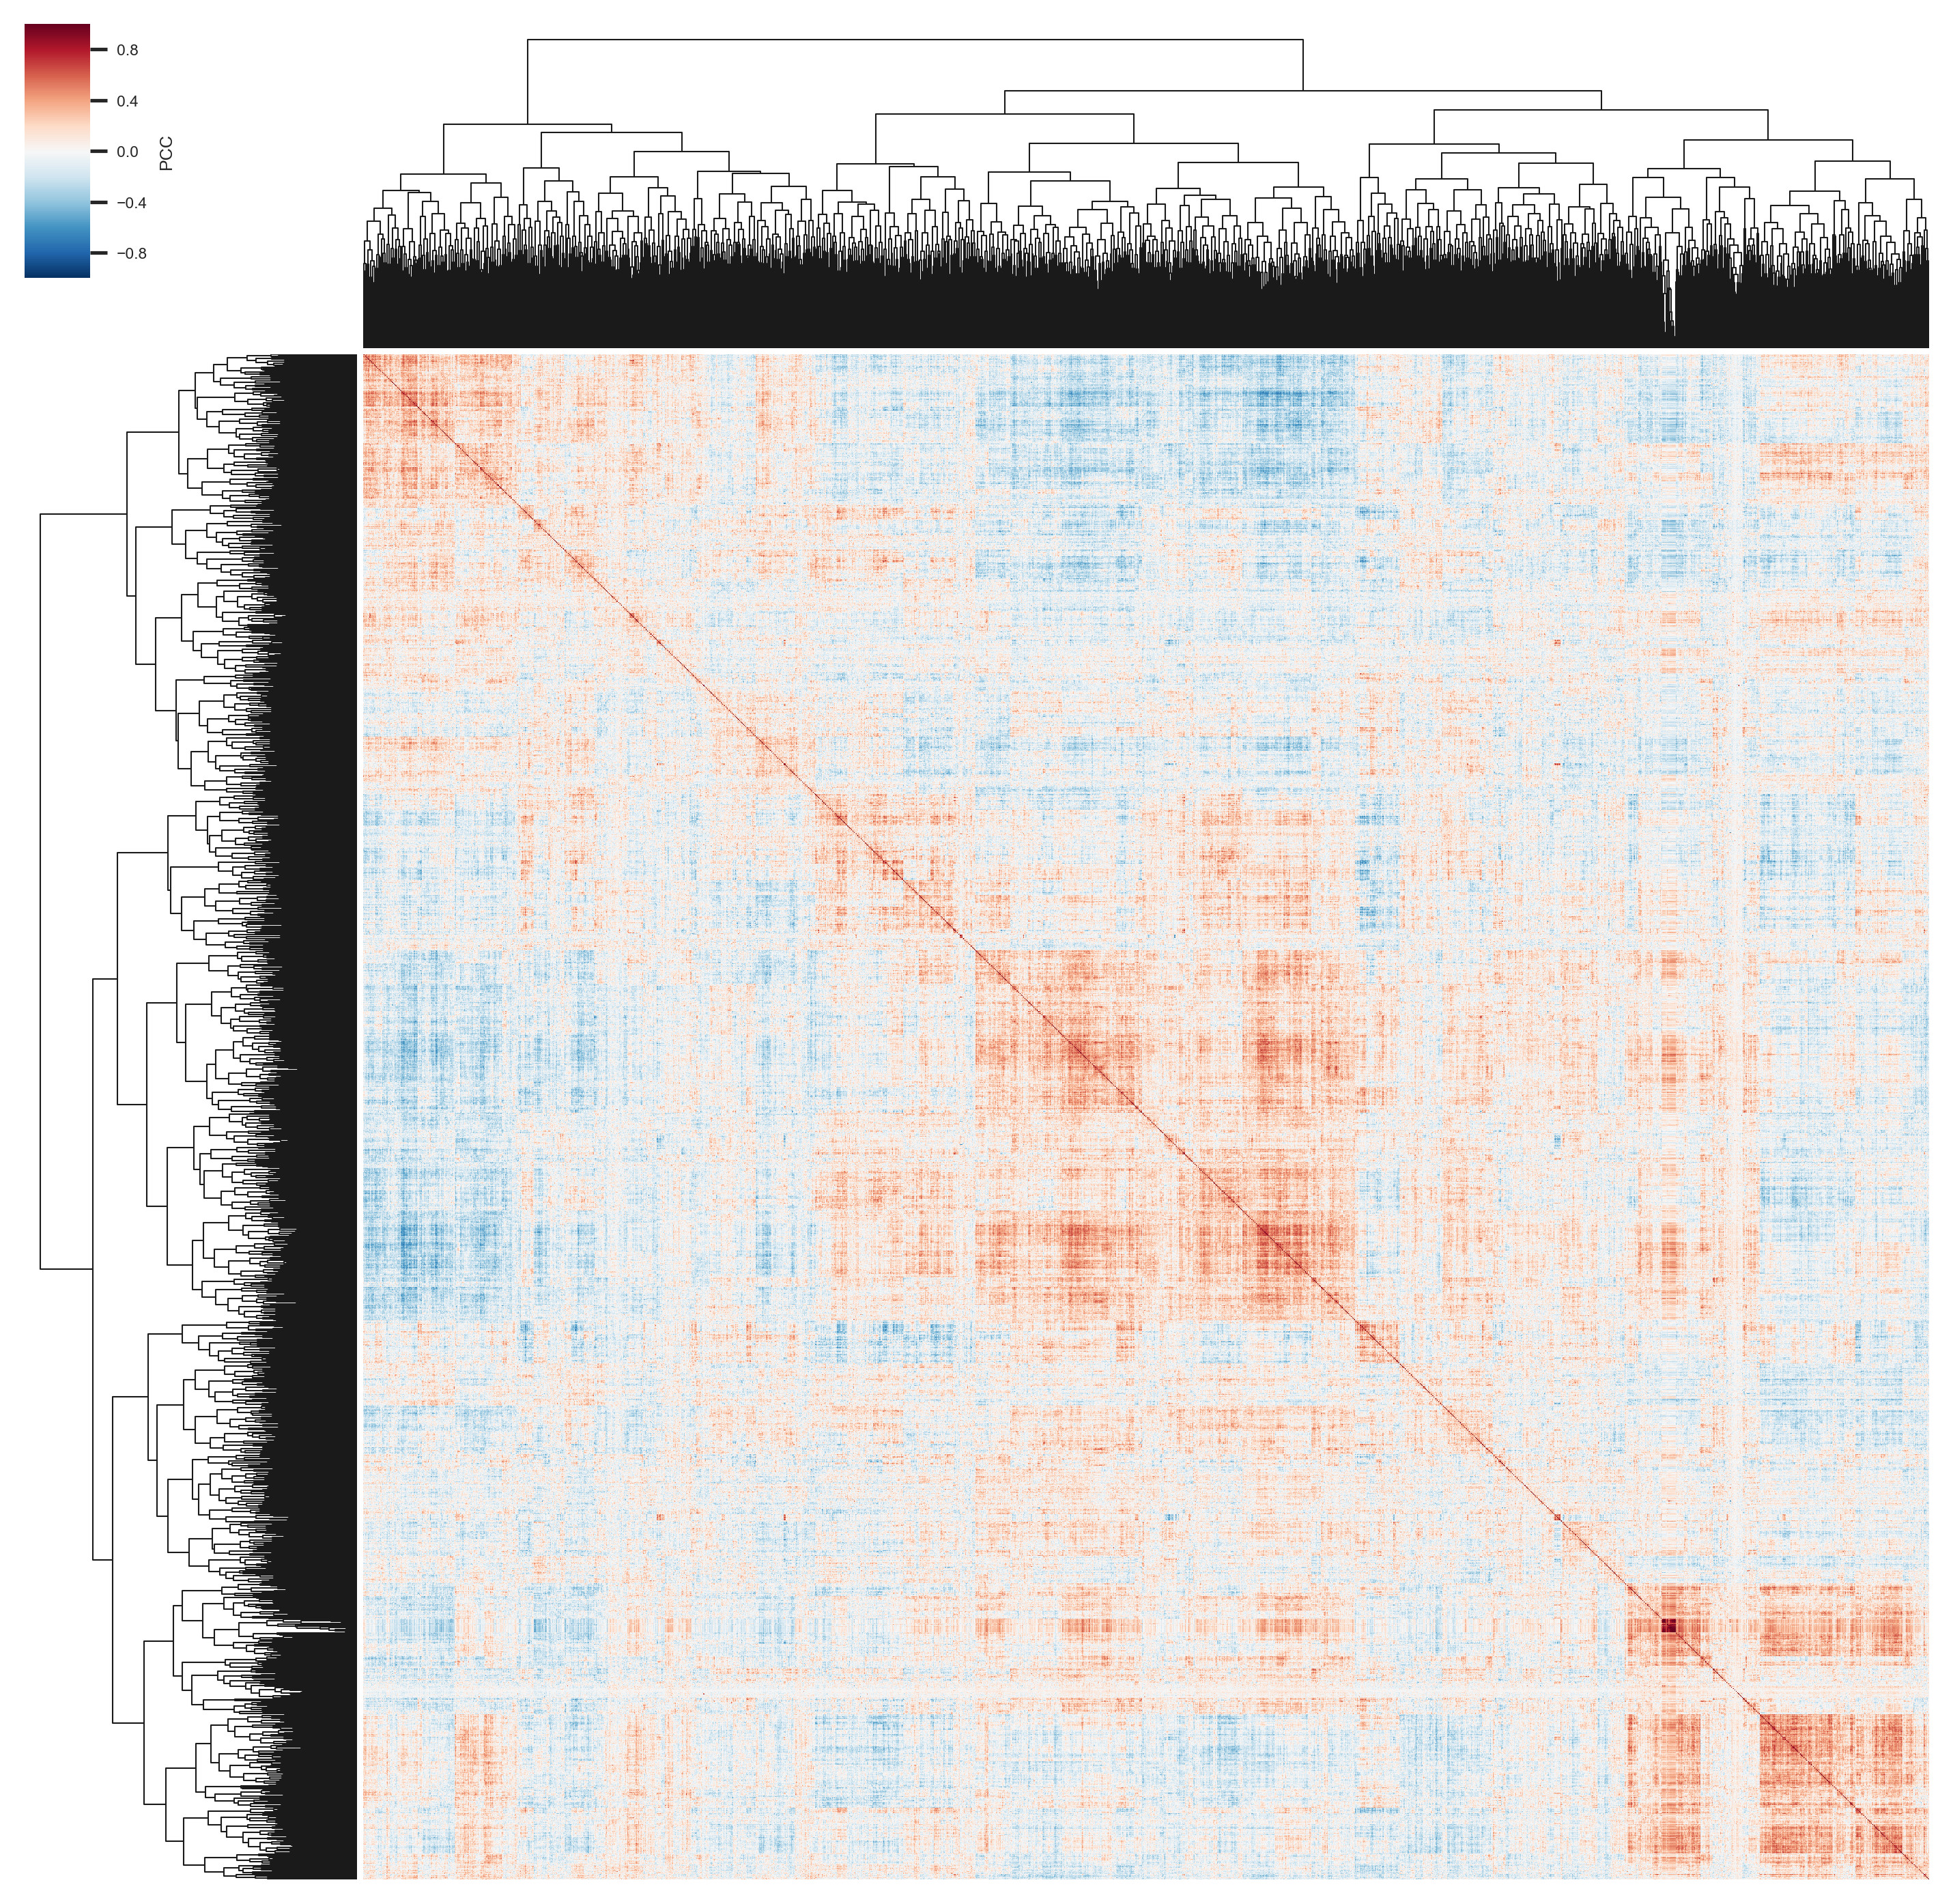
\includegraphics[width=\textwidth]{./Chapter_yeast/clustermap_ids}
    \caption{%
        Correlation of strains.
        The Pearson correlation coefficient (PCC) matrix of strains across all conditions was clustered using UPGMA.
    }
    \label{fig:clustermap-ids}
\end{figure}

\section{Significance testing to identify significant phenotypes}

Strains whose growth were affected in particular conditions were identified using null hypothesis significance testing. Absence of knocked out genes may affect growth, regardless of the condition, and in particular may have a negative affect on growth, as suggested by the mean colony size of $-0.046$ that we measured across all strains and conditions. To account for these effects, the null distribution for each strain is the distribution of its colony sizes in plain media at $32$$^{\circ}$C: `YES\_32' for conditions based on YES media, or `EMM\_32' for EMM media. For each strain and condition, the colony size distribution was compared to its corresponding null distribution using the two-sample unequal variance t-test (also known as Welch's test). The null hypothesis was that there is no difference between how a strain grows in a condition and its corresponding control condition. We used the two-sample unequal variance t-test because colony sizes of strains grown in the control condition follow a distribution, and this distribution might not have the same variance as non-control conditions.

Conditions are independent of other conditions. We considered each condition to be a separate experiment, so applied multiple testing correction to $P$ values from each condition separately \cite{Bourgon2010}. We believe that it makes more biological sense to consider each condition a separate experiment and not each strain as a separate experiment. In total, \num{10318} hits were called at the $Q < 0.01$ significance level (\ref{fig:significance-testing-p-values}). $128$ out of the $131$ conditions had at least one hit, with a median of $43$ hits per condition (\ref{fig:significance-testing-hits-per-condition}). Other than the two control conditions, the only other condition that had no hits was `YES\_Diamide\_3mM' because only one repeat was performed for this condition because it was too toxic.
\num{3058} strains out of \num{3510} strains that we screened had at least one hit, with a median of $2$ and a mean of $3$ hits per strain (\ref{fig:significance-testing-hits-per-id}). Eight strains had hits in more than $20$ conditions (\ref{table:hits-per-id}), consisting of transcription factors, kinases (protein kinase gsk3 and serine/threonine-protein kinase cds1) and a critical metabolic enzyme (fructose-1,6-bisphosphatase).

\begin{table}[hbt!]
    \centering
    \caption{%
        Number of hits per strain.
    }
    \label{table:hits-per-id}
    \begin{tabular}{lllc}
        \toprule
        \textbf{Gene ID} & \textbf{Symbol} & \textbf{Gene long name} & \textbf{No. hits} \\
        \midrule
        SPBC106.10 & pka1 & cAMP-dependent protein kinase & $97$ \\
        SPBC725.11c & hap2 & Transcriptional activator hap2 & $78$ \\
        SPBC1105.14 & rsv2 & Zinc finger protein rsv2 & $70$ \\
        SPBC29B5.01 & atf1 & Transcription factor atf1 & $64$ \\
        SPBC1198.14c & fbp1 & Fructose-1,6-bisphosphatase & $54$ \\
        SPAC1687.15 & gsk3 & Protein kinase gsk3 & $50$ \\
        SPCC18B5.11c & cds1 & Serine/threonine-protein kinase cds1 & $36$ \\
        Wild type & - & - & $30$ \\
        \bottomrule
    \end{tabular}
\end{table}

\begin{figure}[!phbt]
    \centering
    \begin{subfigure}{0.75\textwidth}
        \centering
        \includegraphics[width=\textwidth]{./Chapter_yeast/significance_testing_p_values_histogram}
        \caption{%
            Testing whether strain growth is significantly affected by conditions.
        }
        \label{fig:significance-testing-p-values}
    \end{subfigure}
    ~
    \begin{subfigure}{0.49\textwidth}
        \centering
        \includegraphics[width=\textwidth]{./Chapter_yeast/significance_testing_hits_per_condition_histogram}
        \caption{%
            Number of hits per condition.
        }
        \label{fig:significance-testing-hits-per-condition}
    \end{subfigure}
    ~
    \begin{subfigure}{0.49\textwidth}
        \centering
        \includegraphics[width=\textwidth]{./Chapter_yeast/significance_testing_hits_per_id_histogram}
        \caption{%
            Number of hits per strain.
        }
        \label{fig:significance-testing-hits-per-id}
    \end{subfigure}

    \caption{%
        Significance testing.
        \textbf{a.}
        Testing whether strain growth is significantly affected by conditions.
        The null hypothesis was that there is no difference between how a strain grows in a condition and its corresponding control condition---‘YES\_32’ for conditions based on YES media, or ‘EMM\_32’ for EMM media.
        Two-sample unequal variance t-tests were performed for colony size distributions and their corresponding null distributions.
        \textbf{b.}
        Number of hits per condition.
        Two-sample unequal variance t-tests were performed for colony size distributions and their corresponding null distributions.
        $P$ values were corrected for multiple testing using the Benjamini-Hochberg method.
        Hits were called at the $Q = 0.01$ significance level.
        \textbf{c.}
        Number of hits per strain.
        Two-sample unequal variance t-tests were performed for colony size distributions and their corresponding null distributions.
        $P$ values were corrected for multiple testing using the Benjamini-Hochberg method.
        Hits were called at the $Q = 0.01$ significance level.
    }
\end{figure}

% Separate figs of the subfig version above
%
% \begin{figure}[!hbt]
%     \centering
%     \includegraphics{./Chapter_yeast/significance_testing_p_values_histogram}
%     \caption{%
%         Testing whether strain growth is significantly affected by conditions.
%         The null hypothesis was that there is no difference between how a strain grows in a condition and its corresponding control condition---‘YES\_32’ for conditions based on YES media, or ‘EMM\_32’ for EMM media.
%         Two-sample unequal variance t-tests were performed for colony size distributions and their corresponding null distributions.
%     }
%     \label{fig:significance-testing-p-values}
% \end{figure}
%
% \begin{figure}[!hbt]
%     \centering
%     \includegraphics{./Chapter_yeast/significance_testing_hits_per_condition_histogram}
%     \caption{%
%         Number of hits per condition.
%         Two-sample unequal variance t-tests were performed for colony size distributions and their corresponding null distributions.
%         $P$ values were corrected for multiple testing using the Benjamini-Hochberg method.
%         Hits were called at the $Q = 0.01$ significance level.
%     }
%     \label{fig:significance-testing-hits-per-condition}
% \end{figure}
%
% \begin{figure}[!hbt]
%     \centering
%     \includegraphics{./Chapter_yeast/significance_testing_hits_per_id_histogram}
%     \caption{%
%         Number of hits per strain.
%         Two-sample unequal variance t-tests were performed for colony size distributions and their corresponding null distributions.
%         $P$ values were corrected for multiple testing using the Benjamini-Hochberg method.
%         Hits were called at the $Q = 0.01$ significance level.
%     }
%     \label{fig:significance-testing-hits-per-id}
% \end{figure}

\subsection{Assigning fission yeast proteins to FunFams}

\emph{S. pombe} proteins were mapped to FunFams, to encode homolog information when using machine learning to predict GO annotations. Sequences of the \num{5137} proteins encoded in \emph{S. pombe}'s genome were scanned against HMMs from each of the \num{68065} FunFams. At a threshold of E $< 10^{-3}$, \num{3319} ($64\%$) proteins had \num{149099} hits to \num{23900} FunFams ($35\%$).
\num{10136} of these FunFams ($42\%$) were hit by only one protein (\ref{fig:hits_per_funfam}). The median number of hits per FunFam was $2$ and the mean was $5.35$.
The maximum number of hits per FunFam was $126$ proteins for the WD40 repeat-containing serine/threonine kinase FunFam from the YVTN repeat-like/Quinoprotein amine dehydrogenase superfamily (2.130.10.10/FF/102735).

\begin{figure}[!hbt]
    \centering
    \includegraphics{./Chapter_yeast/hits_per_funfam_histogram}
    \caption{%
        Number of hits per FunFam for \emph{S. pombe} proteins.
        Proteins were scanned against the CATH v4.2 FunFam HMM library using an E-value threshold of E $< 10^{-3}$.
        Only FunFams with at least one hit are shown.
    }
    \label{fig:hits_per_funfam}
\end{figure}

We associated GO terms to FunFams by identifying all GO terms that are annotated to proteins in each FunFam (\ref{fig:funfams_per_go_slim_term}). FunFams were associated with GO Slim terms with a median of \num{1619} across the $53$ \emph{S. pombe} GO Slim terms. `Vesicle mediated transport' (GO:0016192) was associated with the maximum number of \num{11279} FunFams. Non-parametric testing, using the number of descendants each term has as the null distribution, indicates that `vesicle mediated transport' has significantly more descendant terms than expected, $P = 0.011$, which may go some way to explain why $17\%$ of FunFams contain sequences that are annotated with terms related to `vesicle mediated transport'.

\begin{figure}[!hbt]
    \centering
    \includegraphics{./Chapter_yeast/funfams_per_go_slim_term}
    \caption{%
        Numbers of FunFams associated with GO Slim terms.
        GO terms were associated to FunFams by identifying all GO terms that are annotated to proteins in each FunFam.
        All annotations were included, except those with NAS, ND, TAS or IEA evidence codes, but UniProtKB-kw IEA curated terms were included.
        Ancestor terms that have ‘is\_a’, ‘has\_part’, ‘part\_of’ and ‘regulates’ relationships were also included.
    }
    \label{fig:funfams_per_go_slim_term}
\end{figure}

\subsection{Benchmarking machine learning protein function prediction models}

GO Slim terms for \emph{S. pombe} were predicted using RFs and the one-vs-rest classification strategy. Different combinations of features were used to predict GO Slim terms and their performance was evaluated (\ref{fig:pr-go-slim}). The prediction error was estimated using five independent repeats of $5$-fold cross-validation. We present the results for models trained using one type of data first and then go on to discuss models trained using a combination of different data.

\begin{figure}[!hbt]
    \centering
    \includegraphics[width=0.9\textwidth]{./Chapter_yeast/micro-averaged_PR}
    \caption{%
        Precision-recall curves for predicting GO Slim terms.
        The 53 GO Slim terms were predicted using RFs and a one-vs-rest classification strategy.
        The prediction error was estimated using five independent repeats of $5$-fold cross-validation.
        Precision-recall curves are plotted for each repeat (thin translucent curves) as well as a micro-averaged curve (thick solid curves).
        Numbers in legend correspond to the micro-averaged AUPR.
        Legend abbreviations: GP, growth phenotypes; NE, network embeddings; FF, FunFam homology data.
    }
    \label{fig:pr-go-slim}
\end{figure}

\ref{chapter:network-fusion} reported how deepNF \cite{Gligorijevic2018}---a state of the art gene function prediction method---was applied to \emph{S. pombe} networks to predict GO terms.
Here, we used the best $256$D network embeddings from \ref{chapter:network-fusion} as features to predict GO Slim terms. Alone, network embeddings were the best set of features (AUPR $= 0.583$; yellow curve). The next best features were FunFam homology data (AUPR $= 0.424$; orange curve). Third best were the yeast growth phenotype data (AUPR $= 0.126$; light blue curve). At first glance, this performance may not appear so good, however, the classifier is many times better than random. \emph{S. pombe}'s GO Slim annotations have $|\text{P}|= \num{7646}$ and $|\text{N}|= \num{224706}$, so a random classifier would have AUPR $= 0.0329$. Therefore, these growth phenotype data are able to predict GO Slim terms $3.8$ times better than a random classifier, but, compared to network embeddings and FunFam data, the growth phenotypes are poorly predictive of GO Slim annotations.

Two combinations of features were tested. A combination of network embeddings and FunFam data produces a performance $3\%$ higher than the network embeddings alone (AUPR $= 0.599$; green curve). Due to the way that we performed the cross-validation, this is a genuine---albeit modest---increase in performance. Another combination of growth phenotypes and network embeddings produces a performance $7\%$ lower than the network embeddings alone (AUPR $= 0.544$; dark blue curve).

\subsection{Annotating fission yeast proteins with new functions}

GO terms that are annotated to between \numrange{50}{1000} \emph{S. pombe} proteins were predicted with AUPR $= 0.569$ (\ref{fig:predict_GO_pr}). \num{2390915} annotations were predicted, of which \num{97017} were already known and in the target set. After removing known annotations, with experimental or curated evidence codes, and \num{2167057} predictions with probability $P(\text{annotation}) < 0.1$, \num{126841} predictions remained for $534$ GO terms in \num{4456} proteins.
Only \num{2628} ($2\%$) of these predictions were present in the \emph{S. pombe} GO annotations with IEA evidence codes, and \num{7710} ($6\%$) with IEA, NAS or ND evidence codes. We do not predict any functions for proteins that had no annotations (regardless of evidence codes), and we also do not predict functions of proteins that had no experimental or curated annotations (i.e. only IEA, NAS or ND evidence codes). We do, however, predict \num{117654} new functions for proteins that previously had experimentally validated functions.

\begin{figure}[!hbt]
    \centering
    \includegraphics[width=0.9\textwidth]{./Chapter_yeast/predict_GO_pr}
    \caption{%
        Performance of predicting functions of \emph{S. pombe} proteins.
        The model was trained on network embeddings and FunFams.
        GO terms that are annotated to between \numrange{50}{1000} proteins are included.
        A precision-recall curve is plotted.
        Numbers in legend correspond to the micro-averaged AUPR.
    }
    \label{fig:predict_GO_pr}
\end{figure}

$692$ \emph{S. pombe} proteins have unknown function, of which $409$ have orthologues in other organisms and $145$ of these are conserved in vertebrates---the so called `priority unstudied genes' defined by PomBase. (NB some `unknown function' and `priority unstudied' proteins have automatically assigned functions with the IEA evidence code.) We analysed the functions that were predicted for proteins conserved in vertebrates and the priority unstudied proteins (accessed on June 10, 2020). For the conserved proteins, we predicted \num{4285} functions for $397$ GO terms in $153$ proteins ($22\%$). $18$ of these annotations were previously predicted with IEA evidence codes. For the priority unstudied proteins, we predicted \num{1865} functions for $350$ GO terms in $64$ ($44\%$) proteins. $18$ of these annotations were previously predicted with IEA evidence codes. $133$ of the $145$ priority unstudied proteins are in the Bioneer gene deletion mutant library, and $60$ out of the $64$ priority unstudied proteins that we predicted functions for are in the Bioneer collection.

\subsection{CAFA 4}

We entered CAFA 4 with predictions for fission yeast GO terms, under the team name `OrengoFunFamLab2'. We experimented with many different combinations of features and submitted the three models that had the best AUPR from cross-validation (\ref{fig:cafa-pr}). Our three models were all trained on network embeddings. Additionally, v4.3 FunFams were used in model 1 and v4.2 FunFams were used in model 2. Our initial model---using network embeddings and v4.3 FunFams---produced AUPR $= 0.473$ (results not shown). After extensive experimentation (results not shown), we were able to to increase the AUPR of our final models considerably. Despite this, model performance appears to be asymptotic to AUPR $\approx 0.58$.

\begin{figure}[!hbt]
    \centering
    \includegraphics[width=0.9\textwidth]{./Chapter_yeast/cafa_pr}
    \caption{%
        Performance of three models submitted to CAFA 4.
        Models were trained on different combinations of network embeddings (NE) and FunFams (FF).
        Precision-recall curves are plotted.
        Numbers in legend correspond to the micro-averaged AUPR.
    }
    \label{fig:cafa-pr}
\end{figure}

We can understand how the various features contribute to the models by analysing the shape of precision-recall curves. Network embeddings produce high precision predictions at low recall, whereas, FunFams increase the precision of predictions at high recall. If the goal is to assign functions to a set of proteins, without making any incorrect predictions, or missing any predictions, then it may be beneficial to use FunFam information, possibly in combination with network embeddings.

Though not directly relevant to this chapter, I also participated in the Orengo group's FunFam-based predictions for all $18$ species, under OrengoFunFamLab team's 1, 3, 4 and 5. The preliminary results of CAFA 4 were presented at the ISMB conference in July 2020. For each ontoloy, the top 10 methods were presented, where each research group could only occur once in the top 10. The OrengoFunFamLab3 method came top in molecular function, third in biological process, and was not placed in the top 10 for cellular component. OrengoFunFamLab3 used CATH v4.3 and InterPro data to train an XGBoost classifier using a learning to rank strategy.


\section{Discussion}

\subsection{Many factors may contribute to colony size phenomics being unreliable}

Colonies of \emph{S. pombe} gene deletion mutants displayed a high false negative rate for phenotypes in conditions and some strains had a high variance in colony sizes in particular conditions (\ref{sec:Estimating the reliability of colony sizes}). We assessed the variance in measuring colony sizes, due to technical errors associated with scanning plates, and found it to be very low. We normalised colony sizes to account for spatial biases, and the position of strains relative to each other, associated with plates. Therefore, false negative phenotypes appear to be genuine biological phenomena, which could have many contributing factors, including:

\begin{itemize}
    \item viability of cells after thawing the gene deletion mutant collection,
    \item number of cells pinned on the plate to seed each colony,
    \item temperature and other environmental conditions of the laboratory during preparation of plates,
    \item temperature and other environmental conditions in the incubator during growth,
    \item nutrients and their concentrations within the agar plate.
\end{itemize}

The Bioneer collection contains gene deletion mutant strains of \emph{S. pombe} for all non-essential genes. Genes may be non-essential because of genetic redundancy, or because the gene is not required in benign standard laboratory growth conditions. By stressing gene deletion mutants in a panel of growth conditions, we hoped to trigger condition-dependent reduced fitness (slow growth) or condition-dependent essentiality (no growth) of the deleted genes. Genetic redundancy creates alternative routes for flux through metabolic and signalling pathways. \emph{S. pombe} has not undergone whole-genome duplications \cite{Vo2016}, unlike \emph{S. cerevisiae} \cite{Kellis2004}, but instead its paralogs arose from small-scale duplications of chromosome regions. Whole-genome duplications give rise to paralogs with redundant functions, whereas, paralogs from small-scale duplications tend to be functionally divergent \cite{Hakes2007} or subfunctionalised \cite{Force1999,Stoltzfus1999}. As such, it is reasonable to think that \emph{S. pombe} would not exhibit much genetic redundancy---after all, carrying two genes that perform the same function is a fitness cost. However, we have previously shown that \emph{S. pombe} rewires its gene expression and protein interaction networks after stress, to introduce redundancy and increase resilience to mutation \cite{Lehtinen2015a,Lehtinen2013}. By subjecting \emph{S. pombe} to stressful conditions, instead of eliciting phenotypes, we may have inadvertently triggered it to become more tolerant.

Data from multiple, independent repeats are often processed to obtain a point estimate that estimates the population distribution. A measure of central tendency, like the mean or median, is usually taken. If the false negative rate for phenotypes is caused by an underlying stochastic mechanism, or a mechanism that we perceive as stochastic, then central tendencies will obfuscate any true positives. For example, consider four colonies with sizes ${[}-1.0, -0.1, 0.0, 0.1{]}$, where $-1.0$ is a true positive and $-0.1$, $0.0$ and $0.1$ are false negatives. Here, the mean is $-0.25$ and the median is -$0.05$, which would both fail to capture the ground truth phenotype. To combat the high false negative error rate, we took as point estimates the maximum observed effect size from any repeat. That is, in our toy example above, the point estimate is -$1.0$, which successfully captures the ground truth phenotype. The downside of this approach is the possibility of increasing the false positive rate, which may arise if, for example, the grid normalisation failed to adequately normalise a plate's spatial biases. False positives are not as detrimental as false negatives. False positives can be filtered out by experimental screening or using evidence from the literature, but false negatives will not be tested because they would not be in the set of predicted functions.

\subsection{FunFams were used to encode homology information in a novel way for machine learning}

This is the first time that FunFam homology information has been used by us in a machine learning context. We encoded this information as a matrix of log-transformed HMM E-values. The resulting matrix is high-dimensional and sparse. HMM-based features have been used previously to predict protein function with machine learning \cite{Cheng2006,Shah2008,Dlakic2009,Lees2017,Zaman2017}, including logarithms of E-values \cite{Cheng2006}. High-dimensionality and sparsity are not ideal properties for machine learning, but we attempted to mitigate their negative effects using a novel training strategy that, to our knowledge, has never been used before. We trained models using the one-vs-rest strategy and only included FunFams that are associated with the GO term being predicted, thus reducing the dimensionality of the feature space (\ref{fig:funfams_per_go_slim_term}). When this work was conducted, deepNF was one of the best function prediction methods \cite{Gligorijevic2018}, so it was encouraging to see that the FunFams were able to improve on deepNF's performance.

All GO Slim terms are in the `biological process' ontology. Network-based features were more predictive of GO Slim terms than FunFam-based features. At least two factors may contribute to this phenomenon. First, FunFams are groups of functionally pure proteins from different species, therefore they tend to be better at predicting GO terms from the `molecular function' ontology, rather than the `biological process' ontology \cite{Jiang2016,Zhou2019}. In CAFA 3, for example, the Orengo-FunFam team was ranked second place for predicting `molecular function' terms and fourth place for `biological process' terms. Therefore, this may explain only the modest performance improvements achieved when training models using FunFam and network embedding features. Second, \emph{S.pombe} has been characterised extensively, so has comprehensive network data compiled across a large number of separate experiments. It could be that the quality of network data in \emph{S. pombe} is very high and this effect would also be observed in popular model organisms, but not in less well-studied species.

The WD40 repeat-containing serine/threonine kinase FunFam that was hit by the most \emph{S. pombe} proteins is large and contains \num{113743} sequences from UniProt. The inclusion threshold---the HMM's trusted cutoff value---for this FunFam is $6.00$, which is very low and suggests that either the FunFam multiple sequence alignment is poor, or this FunFam is affected by a known bug in CATH v4.2 FunFams. Sequences from a FunFam multiple alignment are scanned against the corresponding FunFam HMM and the lowest bit score is used as the inclusion threshold. We recently discovered a problem that affects some FunFams, whereby short sequences, or subsequences, matched the HMMs with commensurately small bit scores. As such, sequences may be assigned to FunFams erroneously. Despite this, we can be reassured about the false positive rate because $95\%$ of FunFams are hit by no more than $21$ proteins.

\subsection{Network data is powerful at predicting protein function}

Network embeddings were the most predictive set of features for \emph{S. pombe} protein function. We used deepNF to generate low-dimensional embeddings of proteins using information about their context across multiple networks \cite{Gligorijevic2018}. deepNF is a highly competitive protein function prediction method. This is somewhat surprising, given that the method only uses network data. Until recently, network data had a bad reputation for being noisy and incomplete \cite{Sprinzak2003,DeSilva2006,Kuchaiev2009,Zaki2013}, but recent work suggests that networks are now more reliable \cite{Heriche2014,Lehtinen2015,Piovesan2015,Moya-Garcia2017,Gligorijevic2018,You2019}. For example, GOLabeler \cite{You2018} was the best method overall in CAFA 3 \cite{Zhou2019} (Zhu Lab team in CAFA 3), but NetGO \cite{You2019}, a model that adds network data to GOLabeler, was found to improve performance.

It has not escaped our attention that all of the work cited above use STRING \cite{Szklarczyk2019,Szklarczyk2015} as their sole source of network data. The authors state that STRING ``aims to collect, score and integrate all publicly available sources of protein--protein interaction information, and to complement these with computational predictions'' \cite{Szklarczyk2019}. It is conceivable that the power of network data actually results from STRING's coverage, high-quality curation and accurate predictions, because it is known that integrating information from independent sources improves predictions \cite{Lees2011}.

The growth phenotype data were acquired using a high-throughput plate colony size assay. These data constitute a single screen that has associated biological and technical error rates \cite{Bilder2009}, as opposed to STRING \cite{Szklarczyk2019}, which is, in essence, a meta-analysis of all known protein-protein interaction information, with far lower error rates.

%(\ref{fig:network_embedding_clustermap})
It may appear surprising that, when combined with the network embeddings, the growth phenotypes cause a reduction in performance, but this can happen for the following reasons. Firstly, each tree in the forest is trained on random subsets of features from the training data that are selected from $131$ growth phenotypes and $221$ network embedding dimensions,
so the growth phenotypes account for $37\%$ of features. Given that we know growth phenotypes are much less predictive than network embeddings, it is almost surprising that the reduction in performance is not larger than $7\%$, relative to network embeddings alone. Secondly, growing trees uses a greedy algorithm, so the associated error may not be equal to the global minimum, but rather may be an artefact of the heuristics used in the algorithm.

\subsection{On CAFA and its value}

Participating in CAFA 4 was a very valuable academic experience. Developing function prediction methods in isolation, without releasing predictions to the public, is futile. However, not every computational researcher or group is lucky enough to be able to collaborate with experimentalists that can validate their predictions. CAFA, the triennial evaluation of protein function prediction methods, was set up to provide a robust validation, without the need for explicit collaborations. Models are benchmarked on unseen data using a time-delayed evaluation to accumulate new experimentally-validated functions. This is in contrast to CASP \cite{Kryshtafovych2019}, the community benchmark of protein structure prediction methods, which uses newly solved structures to evaluate model performance. In so doing, CAFA acts as a community benchmark of protein function prediction methods and captures the zeitgeist of the data, methods and models that are used to predict protein function.

Some interesting questions were raised during CAFA due to the evaluation strategy: Which models should be developed? To what extent, during development, should model choice be influenced by performance on benchmarks? How can overfitting on benchmarks be avoided, whilst still performing well on the evaluation data set? It is vital to not overfit models to benchmarks because the annotations in benchmarks are unlikely to be representative of the annotations that will accumulate to form the evaluation data set. Instead, models should be developed using general biological principles and our intuition \cite{Gigerenzer2014}. In other words, if a model, that performs well in benchmarking, looks unlikely, it probably is. Here, we stuck to three biological principles that functions are: conserved through evolution (FunFams), encoded in how proteins interact (network embeddings), and functions have phenotypic consequences (growth phenotypes).

Here, we only predicted functions for one of the $18$ model organism proteomes included in CAFA 4. The small number of proteins in the \emph{S. pombe} proteome meant that evaluating the performance of our models using a time-delay strategy was infeasible, so instead we used cross-validation and precision-recall curves. We will have to wait until the final results are due to be published in October to understand how well our models perform. We do not know whether performance is limited by the RF, our training strategy, or inherent inaccuracies and noise in the features and GO term annotations. Either way, CAFA 4 is likely to generate a large number of high-quality predicted functions for fission yeast, which, if made public, could be hosted on PomBase. However, these predictions will need to be validated by the community.

Preliminary results from CAFA 4 suggest that FunFam-based predictors are still cutting edge, especially amongst tough competition from advanced neural network-based predictors. We were delighted to be placed top for molcular function, as we believe FunFams capture molecular function information well. We were also encouraged by achieving third place for biological process, as these terms are harder to predict using the type of information encoded by FunFams. For comparison, in CAFA 3, we were second for molecular function and fourth for biological process.

\subsection{Conclusion}

Here, we trained machine learning models to predict functions of \emph{S. pombe} proteins. We obtained encouraging results from evaluating our models using cross-validation and also entered our predictions into CAFA 4. However, to be confident about the quality of our predictions, we need experimental validation by growing gene deletion mutant strains in conditions that would elicit loss of function phenotypes. We applied our protein function prediction method to fission yeast as a proof of principle, but the method is species-agnostic, providing feature and target data are available for any species of interest. Despite this, our method is time-consuming to train and is restricted to the information from one species at a time. Going forward, methods that are not restricted to a single species may be more preferable, such as deepFRI \cite{Gligorijevic2019}, which aggregates information from any species.

Aetiologies of protein function at the residue-, domain-, molecular-, cellular-, or organism-level remain a partial mystery, but recent developments in the field of protein function have gone some way towards being able to predict functions. We are grateful to have been able to make a small contribution to the field and its development. In the future, a greater emphasis will be placed on de-blackboxification of predictions and on uncovering general principles that explain how proteins are bestowed with functions.
